\chapter{\IfLanguageName{dutch}{Stand van zaken}{State of the art}}%
\label{ch:stand-van-zaken}

% Tip: Begin elk hoofdstuk met een paragraaf inleiding die beschrijft hoe
% dit hoofdstuk past binnen het geheel van de bachelorproef. Geef in het
% bijzonder aan wat de link is met het vorige en volgende hoofdstuk.

% Pas na deze inleidende paragraaf komt de eerste sectiehoofding.

%\lipsum[7-20]

\section{Wie is Lockit Rentals}%
\label{sec:lockitRentals}


Lockit Rentals is een naam onder het bedrijf VD Group BV. Deze is opgericht op 6 november 2019 door Sébastien Vandenhouten en Wannes Van Dorpe met als doel lockers te verhuren op evenementen. Enkele maanden na de oprichting begon de covid-19 crisis die de volledige sector tot stilstand deed komen. Na de crisis werd er direct geïnvesteerd in nieuwe lockers. Niet de gewone traditionele lockers, maar speciale technologische lockers die nog niet beschikbaar waren in België. De lockers werden in een mum van tijd omgebouwd tot QR-smart locker units met daarin lockers. Zo zijn er in het voorjaar van 2022, 13 units geproduceerd door Lockit Rentals. Op de dag van vandaag wordt er ijverig gezocht naar nieuwe investeerders om hun vloot van units uit te breiden.

Er zijn verschillende manieren om smart lockers systemen te gaan produceren. Hieronder volgt een opsomming van de verschillende smart lockers systemen elk met hun eigenschappen. Deze methodes zijn opgesteld door Lockit Rentals om hun marktonderzoek te starten.
\\
\textbf{Pincode:}
\begin{itemize}
    \item Kan vergeten worden
    \item Manuele verkoop mogelijk
    \item 100\% online verkoop mogelijk
    \item Trage verwerking bij openen van locker (pincode moet manueel worden ingetypt)
    \item Spieken is mogelijk waardoor er risico’s tot diefstal    
\end{itemize}
    
\newpage
\textbf{Rfid Badge:}
\begin{itemize}
    \item Kan verloren gaan
    \item Manuele verkoop mogelijk
    \item Geen online verkoop mogelijk
    \item Snelle verwerking bij openen locker (scan en go)
    \item Spieken is niet mogelijk
    \item Fysiek object nodig + aankoop kost van badges    
\end{itemize}

\textbf{QR  code:}
\begin{itemize}
    \item Kan niet vergeten worden (kan ook niet onthouden worden)
    \item Manuele verkoop mogelijk
    \item 100\% online verkoop mogelijk
    \item Snelle verwerking bij openen lockers (scan QR-code en go)
    \item Spieken is niet mogelijk
    \item Technisch een veelvoud aan vereenvoudigingen mogelijk    
\end{itemize}

Uit deze korte opsomming van eigenschappen heeft Lockit Rentals besloten om zich te richten op het maken van lockers die openen op basis van een correcte QR code. Het gebruik van een QR code is vandaag de dag ook geen onbekend terrein. Door het mainstream maken van QR codes in betalingen, doorlinken van websites, covidsafe app, etc. zijn veel mensen al eens in aanraking gekomen met een QR-code \autocite{Belle2023}. Het gebruik van een QR code voor het openen van lockers is de logische stap voorwaarts \autocite{Lo2014}.
Uiteraard zijn ze niet de enige die smart locker systemen op de markt hebben. Enkele bedrijven die hier ook bij aanschuiven zijn, mobile lockers, LockerKing en Rental Group.

\section{Hoe zijn de QR-units opgebouwd?}%
\label{sec:QR-units}
De smart locker systemen zijn toegankelijk met een geldige toegangscode die voorgesteld wordt als een QR-code. Het systeem bestaat uit verschillende soorten technologieën en elektronische componenten. De combinatie van hardware en software die nauw met elkaar samenwerken, vormen gezamenlijk één QR-unit \autocite{Jadhav2016} . De units hebben enkel 230 volt nodig om volledig operationeel te zijn. 

De hardware bestaat uit mechanische onderdelen zoals een deurslot \ref{fig:lockerSlot}, het volledige frame van de unit maar ook uit elektronische onderdelen zoals een camera, Raspberry Pi, scherm, etc. De mobiele applicatie waar de QR-codes kan verkocht worden en zo ook genereren, heeft geen verband met de interne werking van een QR-unit. Het enige dat de QR-unit nodig heeft, is een correct opgebouwde QR-code. Hiermee krijgt de festivalganger toegang tot zijn/haar gehuurde locker.

Elke unit bevat 128 lockers verspreid over 4 kasten zoals te zien op figuur \ref{fig:lockerUnit}. De Locker units zijn waterdicht en dus optimaal voor plaatsing in niet overdekte locaties. Eén locker kast bevat 24 lockers, 4 grote die zich op de bovenste rij bevinden. De 20 overige zijn een iets kleiner formaat en situeren zich onderaan. De lange zijden van een QR-unit zijn uitklapbare luiken met aan elke kant twee kasten. Er zijn 4 kasten per unit aanwezig wat een totaal geeft van 128 lockers voorgesteld op figuur \ref{fig:lockerUnit} en  \ref{fig:lockerUnit2}.

\begin{figure}[h]
    \centering
    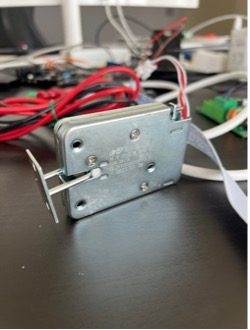
\includegraphics[height=7cm]{F1_lockerSlot.jpg}
    \captionsetup{justification=centering, singlelinecheck=false}    
    \caption{Een locker slot.}
    \label{fig:lockerSlot}
\end{figure}}

\begin{figure}[h]
    \centering
    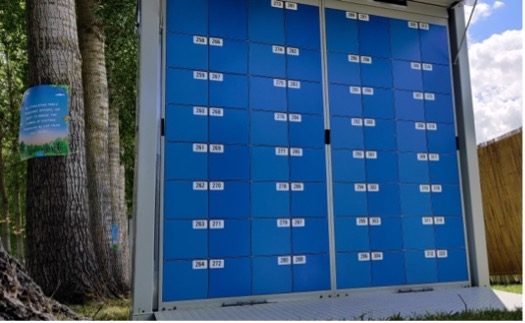
\includegraphics[height=6cm]{F2_lockerUnit.jpg}
    \captionsetup{justification=centering, singlelinecheck=false}    
    \caption{Reële weergave van een locker unit.}
    \label{fig:lockerUnit}
\end{figure}

\begin{figure}[h]
    \centering
    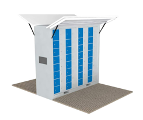
\includegraphics[height=7cm]{F3_lockerUnit2.png}
    \captionsetup{justification=centering, singlelinecheck=false}    
    \caption{Een uitgetekende weergave van een locker unit.}
    \label{fig:lockerUnit2}
\end{figure}}

\section{Hoe is een QR-code opgebouwd?}%
\label{sec:opbouwQR-code}

Een QR-code is een machinaal leesbaar optisch label met informatie over het bijhorende product \autocite{Chang2014}. In deze context wordt het product als toegangscode gebruikt. QR-code staat voor Quick Response code en is een matrix van de welbekende streepjes code \autocite{Tiwari2016}. Het is een tweedimensionale code die informatie zoals tekst, URL of andere data bevat  \autocite{Shin2012} \autocite{Baharav2013}. In ons geval is het dus informatie die toebehoort bij een overeenkomstige locker. De QR-code is zodanig ontworpen dat ze door een smartphone uitgelezen kan worden aan hoge snelheden \autocite{Tiwari2016}. Dit maakt het optimaal als de QR-code gebruikt wordt als toegangscode \autocite{Narang2012}. De grootte van de QR-code kan aangepast worden naarmate de hoeveelheid data die hierin gestockeerd moet worden \autocite{Tiwari2016}. 
\\
Een QR-code wordt opgebouwd en voorgesteld als een vierkant \autocite{Fujita2011}. Hierrond bevindt zich een witte omranding. Dit vormt een contrast zodat de QR-scanner minder moeite heeft om de oppervlakte uit te lezen \autocite{Wang2015}. Dit is 1 van de 7 cruciale eigenschappen. Plaats markeringen zijn aanwezig om de scanner een duiding te geven hoe de code is gepositioneerd. Uitlijnmarkeringen hebben eveneens dezelfde functie maar deze zijn meer van toepassing bij grote QR-codes. De QR-code bevat timing patronen, dit zijn lijnen die de scanner vertellen hoe groot de data matrix is. De twee belangrijkste elementen van een QR-code zijn gegevens en foutcorrectiesleutels. Hierin zit de data gecapteerd inclusief de informatie hoe het algoritme moet omgaan met fouttolerantie \autocite{Tiwari2016}  \autocite{Petrova2016}  \autocite{Li2018}). Een visuele weergave is tezien op \ref{fig:voorstellingQR}. 
De fouttolerantie is doorslaggevend indien de QR-code gebruikt wordt als toegangscode \autocite{Tiwari2016}.  De fouttolerantie kan ingesteld worden door configuratie toe te passen. Het kan ingesteld worden op vier levels beginnend bij fouttolerantie van 7\% tot 30\% \autocite{Tiwari2016}.

\begin{figure}[h]
    \centering
    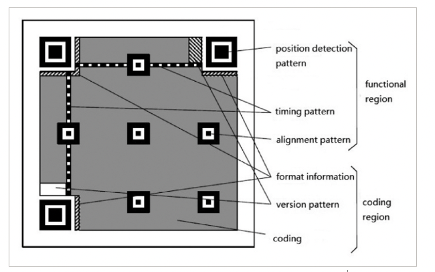
\includegraphics{F4_voorstellingQrCode.png}
    \captionsetup{justification=centering, singlelinecheck=false}    
    \caption{Een technische voorstelling van een QR-code.}
    \label{fig:voorstellingQR}
\end{figure}}

De voordelen van de QR-codes vormen een duidelijk beeld waarom Lockit Rentals voor deze technologie gekozen heeft. Niet enkel naar functionaliteit en flexibiliteit toe maar eveneens is het een makkelijk traceerbare tool. Bij verkoop van QR-codes kan men een overzicht opmaken hoeveel QR-codes er effectief gegenereerd zijn. Op basis van deze gegevens kunnen verkoopcijfers makkelijk berekend worden. 

De kans op diefstal wordt ook alsmaar kleiner als de toegangscode bestaat uit elementen die niet waarneembaar zijn \autocite{Baharav2013}. Hoe minder de persoon in kwestie weet over de code hoe moeilijker deze is om door te geven aan anderen ook al is het niet hun intentie.
\newpage
\subsection{Opbouwen van QR-codes voor verkoop}%
\label{sec:opbouwQR-codeVerkoop}

De applicatie kan meerdere versies van QR-codes genereren elk met hun eigen doel en eigenschappen. Zo bestaan er QR-codes die de software automatisch updaten of een universele QR-code die automatisch alle lockers kan openen. Deze functionaliteit wordt gebruikt voor de lockers te controleren na elk evenement. 

Hoewel een QR-code een standaard grafische voorstelling is, kan de grootte van een code verschillen. Wanneer een code groter is, ontstaat er meer witruimte tussen de pixels \autocite{Li2018}. Hierdoor kan de camera de code makkelijker en sneller scannen \autocite{Karrach2020}. Ook de foutcorrectie zorgt ervoor dat de resolutie vergroot zal worden. Hoe groter de resolutie van de QR-code hoe meer data gestockeerd kan worden \autocite{Chow2016}. 

De reservatie en tot stand brengen van een QR-code zijn twee aparte concepten. Het systeem is geschreven op basis van flexibiliteit en uitbreidbaarheid.

\subsubsection{De reservatie voor een toegangscode van een locker}%
\label{sec:opbouwQR-codeVerkoop1}

\textit {De toelichting die hieronder weergeven wordt, is een vereenvoudigde voorstelling van de effectieve implementatie. Dit onderdeel van de toepassing is niet het hoofdonderwerp van deze bachelorproef, op deze analogie wordt niet verder ingegaan.}

\vspace{7}
De gegevens van de klant worden opgevraagd als hij/zij een QR-code wenst te kopen. Aan de hand van deze gegevens wordt er een gebruikersaccount automatisch aangemaakt en worden de gegevens bijgehouden \ref{lst:ophalenUser}. Deze aanpak maakt het mogelijk om nadien een koppeling te leggen tussen lockernummer en gebruiker.

\begin{lstlisting}[caption={Ophalen de zopas aangemaakte gebruiker zijn gegevens indien hij in het huur proces terecht gekomen is.}, label={lst:ophalenUser}]
    /**
    * Get the user auth uid
    */
    const userAuthUid: string | undefined = context.auth?.uid;
    
    if (!userAuthUid) {
        functions.logger.error('No authenticated user was found', { data: data });
        throw new functions.https.HttpsError(
        'invalid-argument',
        'Something went wrong authenticating your device.'
        );
    }
    
    /**
    * If this user is registerd, get his info
    */
    let user: User;
    if (context?.auth?.token.email) {
        const userd = await db.collection('users').doc(userAuthUid).get();
        user = userd.data() as User;
    }
\end{lstlisting}

Bij het huurproces van een locker moet een huurder het festival aanduiden waar hij/zij de locker wil huren. Niets sluit uit dat de lockers operationeel zijn op twee verschillende locaties. Daarna heeft de huurder de keuze om het formaat te selecteren en als deze optie beschikbaar is hoelang de huurtijd zal zijn. Echter is het verstrijken van deze details over het geselecteerde evenement noodzakelijk voor de opbouw van de QR-code. De QR-code wordt gegenereerd op basis van de beschikbare lockers die aanwezig zijn op het geselecteerde evenement. De verwijzing naar  implementatie \ref{lst:ophalenEventInfo}.

\begin{lstlisting}[caption={Het informatie ophalen van de geselecteerde locatie. Aan de hand van geselecteerde evenement kan er gegevens uit de databank gehaald worden.}, label={lst:ophalenEventInfo}]
    /**
    * Get more info about the shop
    */
    const shopSnap = await db.collection('shop').doc(data.shopId).get();
    const shop: Shop = shopSnap.data() as Shop;
    
    /**
    * Check if selected option is active in shop
    */
    if (!shop.activeOptions?.find((o) => o.optionId === data.optionId)) {
        functions.logger.error(
        'Attempting reservation creation for non-active option',
        { data: data }
        );
        throw new functions.https.HttpsError(
        'invalid-argument',
        'This option is not yet active.'
        );
    }
    
    /**
    * Get more info about the option and location
    */
    const optionSnap = await db
    .collection('shop')
    .doc(data.shopId)
    .collection('options')
    .doc(data.optionId)
    .get();
    const option: ShopOption = optionSnap.data() as ShopOption;
    
    if (!option) {
        functions.logger.error('Can not find option for id', { data: data });
        throw new functions.https.HttpsError(
        'invalid-argument',
        'Something went wrong.'
        );
    }
    
    const locationSnap = await db
    .collection('shop')
    .doc(data.shopId)
    .collection('locations')
    .doc(option.location)
    .get();
    const location: ShopLocation = locationSnap.data() as ShopLocation;
    
    if (!location) {
        functions.logger.error('Can not find location for id', { data: data });
        throw new functions.https.HttpsError(
        'invalid-argument',
        'Something went wrong.'
        );
    }
\end{lstlisting}

Op voorwaarde dat de gebruiker informatie geldig is en er nog een locker beschikbaar is, zal er een reservatie aangemaakt worden en meteen bewaard worden in een databank. Het code die hiervoor verantwoordelijk is kan je terugvinden hieronder \ref{lst:aanmakenReservatie}.

\begin{lstlisting}[caption={De creatie van een reservatie voor het huren van een locker. Deze reservatie wordt bijgehouden in de databank}, label={lst:aanmakenReservatie}]
    /**
    * Create the reservation
    */
    const createdReservationRef = db
    .collection('shop')
    .doc(data.shopId)
    .collection('reservations')
    .withConverter(converter<ShopReservation>())
    .doc();
    
    await transaction.set(createdReservationRef, {
        id: createdReservationRef.id,
        /**
        * Here we decide if the reservation should be filled asap without payment or if a payment is needed
        */
        status: determineReservationStatus(option, data, context, user),
        customerAuthId: userAuthUid,
        customerOrigin: context.rawRequest.headers.referer,
        customerEmail: data.customerEmail,
        customerName: data.customerName,
        customerPhone: data.customerPhone,
        lockerType: data.lockerType,
        shopId: shopSnap.id,
        shopName: shop.name,
        shopAvatar: shop.avatar,
        optionColor: option.color,
        optionId: optionSnap.id,
        optionLocationId: locationSnap.id,
        optionLocationName: location.name,
        optionName: option.name,
        optionPeriodFrom: option.periodFrom,
        optionPeriodTo: option.periodTo,
        optionType: option.optionType,
        priceToPay: option.pricePerType[data.lockerType],
        manual: !!data.manual,
        reservationCreated: moment().unix(),
    });
    
    return Promise.resolve(createdReservationRef);
});
\end{lstlisting}

\subsubsection{Het betalingsverzoek voor een toegangscode van een locker}%
\label{sec:opbouwQR-codeVerkoop12}

Wanneer de databank een nieuwe reservatie constateert, word er een trigger uitgevoerd. Een trigger is een procedure die verplicht uitgevoerd wordt als een welbepaalde tabel een aanpassing ondergaat \autocite{documentation}. In dit geval is het de tabel ‘reservations’. Deze trigger zal een methode aanroepen het betalingsverzoek gecreëerd mag worden. 
De logistieke medewerkers kunnen huurders helpen indien hun QR-code te hard beschadigd is of als ze hun toegangscode tot de locker verloren zijn. Bij het aanmaken van toegangscodes bij logistieke medewerkers verloopt het proces op een alternatieve wijze.  Deze springen over het betalingsproces en verwerven direct een geldige QR-code. Zonder de aangemaakte betaling veld in de databank op te slaan.  \ref{lst:aanmakenBetaling}

\begin{lstlisting}[caption={Valideerd of er een betaling van toepassing is. Indien nodig creëert het een betaling en bewaard deze in de databank}, label={lst:aanmakenBetaling}]
    /**
    * No action is needed but to move the status along
    */
    if (createdReservation.status === ReservationStatus.NO_PROVIDER_NEEDED) {
        await snap.ref.update({
            status: ReservationStatus.OPEN,
        });
    }
    
    /**
    * A payment is needed
    */
    if (createdReservation.status === ReservationStatus.WAITING_FOR_PROVIDER) {
        const mollieApiKey = process.env.MOLLIE_API_KEY || '';
        
        const mollie = await createMolliePayment(mollieApiKey, createdReservation);
        
        /**
        * Create the payment
        */
        const paymentRef = db
        .collection('shop')
        .doc(createdReservation.shopId)
        .collection('payments')
        .withConverter(converter<ShopPayment>())
        .doc();
        
        await paymentRef.set({
            id: paymentRef.id,
            reservationId: createdReservation.id,
            customerEmail: createdReservation.customerEmail,
            customerName: createdReservation.customerName,
            customerPhone: createdReservation.customerPhone,
            lockerType: createdReservation.lockerType,
            optionColor: createdReservation.optionColor,
            optionId: createdReservation.optionId,
            optionLocationName: createdReservation.optionLocationName,
            optionName: createdReservation.optionName,
            priceToPay: createdReservation.priceToPay,
            shopName: createdReservation.shopName,
            status: ShopPaymentStatus.PENDING,
            provider: PaymentProvider.MOLLIE,
            mollieData: {
                id: mollie.id,
            },
        });
\end{lstlisting}

De tool Mollie is een online betalingsservice deze wordt gehanteerd om de betalingen succesvol af te ronden \autocite{docs2023}. Gelijktijdig met de betaling wordt er een interne teller bijgehouden zodat deze locker geblokkeerd wordt voor andere kopers. Als de betaling niet succesvol is, wordt de locker terug vrijgegeven na een bepaalde periode. De betaling word aangemaakt met de gekende informatie over de gewilde locker \ref{lst:aanmakenBetalingMollie}.

\begin{lstlisting}[caption={Mollie betaling aanmaken met nodige data.}, label={lst:aanmakenBetalingMollie}]
    async function createMolliePayment(
    mollieApiKey: string,
    reservation: ShopReservation
    ): Promise<Payment> {
        const mollieClient = createMollieClient({
            apiKey: mollieApiKey,
        });
        return mollieClient.payments.create({
            amount: {
                value: reservation.priceToPay.toFixed(2),
                currency: 'EUR',
            },
            description:
            reservation.shopName +
            ' | ' +
            reservation.optionName +
            ' | ' +
            reservation.lockerType,
            redirectUrl: reservation.customerOrigin + 'reservations/' + reservation.id,
            webhookUrl:
            reservation.customerOrigin?.includes('localhost') ||
            reservation.customerOrigin?.includes('test')
            ? 'https://europe-west2-lockit-testing.cloudfunctions.net/mollieWebhook'
            : 'https://europe-west2-lockit-435cd.cloudfunctions.net/mollieWebhook',
            metadata: {
                shop: reservation.shopName,
                reservation: reservation.id,
                option: reservation.optionName,
                location: reservation.optionLocationName,
                lockerType: reservation.lockerType,
                customer: reservation.customerName,
                customerEmail: reservation.customerEmail,
                customerPhone: reservation.customerPhone,
            },
        });
    }
    \end{lstlisting}

Bij correcte betaling van de klant, zal de applicatie de desbetreffende creatiemethode aanspreken om dergelijke QR-code te genereren. Deze QR-code bevat een random geselecteerde locker nummer inclusief een tijdspanne waarin de toegangscode geldig is. De status van de reservatie die zich al in de databank bevind word aangepast. Hierdoor weet heel de applicatie dat die bepaalde reservatie betaald is \ref{lst:voltooidebetaling}.


\begin{lstlisting}[caption={Voltooide betaling roept de creatie QR-code methode op. Hierbij gebeurt een status update van de vooraf aangemaakte reservatie.}, label={lst:voltooidebetaling}]
    await db.runTransaction(async (transaction) => {
        /**
        * Find a valid available locker
        * Because we can only compare 10 units with the firestore "IN" clause we have to split up
        */
        
        if (!location?.units) {
            throw new Error('No units assigned');
        }
        
        const availableLockerSnap = await getRandomLockerAvailable(
        transaction,
        db,
        reservation.lockerType,
        location?.units
        );
        if (!availableLockerSnap) {
            logger.error('no-open-locker-found', {
                reservation: reservation,
                option: option,
                location: location,
            });
            throw new Error('NO Open lockers found');
        }
        
        const generatedCode = await generateQrCodeWithRecordOnTransaction(
        transaction,
        {
            lockerNumber: availableLockerSnap.data().number,
            start: option?.periodFrom as number,
            end: option?.periodTo as number,
            color: option?.color as string,
            image: reservation?.shopAvatar,
            location: location?.name,
            periodName: option?.name as string,
            name: reservation?.shopName,
        }
        );
        
        /**
        * update current reservation
        */
        await transaction.update(reservationSnap.ref, {
            status: ReservationStatus.FILLED,
            accessCode: generatedCode,
            lockerNumber: availableLockerSnap.data().number,
        });
\end{lstlisting}


\subsubsection{Creatie QR-code na succesvolle betaling.}%
\label{sec:opbouwQR-codeVerkoop123}

Om de QR-code te tonen op de mobiele applicatie hebben we componenten nodig om de gegenereerde QR-code visueel te tonen \ref{fig:qrCodeGebruiker} \ref{fig:qrCodeAdmin}. Hierdoor kan de koper zowel de code scannen op zijn/haar telefoon als op een afgedrukt kaartje \autocite{Chow2016}.

\begin{figure}[h]
    \centering
    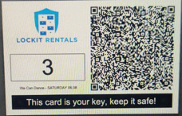
\includegraphics{F5_qrcodeKoper.png}
    \captionsetup{justification=centering, singlelinecheck=false}    
    \caption{Een voorbeeld van een QR-code die gekocht is door een gebruiker voor specifieke lockertoegang op een evenement.}
    \label{fig:qrCodeGebruiker}
\end{figure}}

\begin{figure}[h]
    \centering
    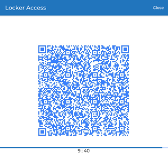
\includegraphics{F6_qrcodeAdmin.png}
    \captionsetup{justification=centering, singlelinecheck=false}    
    \caption{Een voorbeeld van een QR-code die gegeneerd is door een logistieke medewerker met de juiste bevoegdheden voor specifieke lockertoegang op een evenement.}
    \label{fig:qrCodeAdmin}
\end{figure}}

\newpage
Aangezien de generatie van een QR-code dat voorgesteld is als afbeelding wat front-end matige materie is, zal onderstaande code de werking weergeven \ref{lst:qrComponent}. 

\begin{lstlisting}[caption={Typescript code voor een visuele QR-code aan te maken}, label={lst:qrComponent}]
    await db.runTransaction(async (transaction) => {
        export class QrcodeViewerComponent implements OnInit {
            activeQrCode: string = 'EjIQT51wpdf6Is1r+R5+mt8aU0waHVKVK9lzvhXRV4w=';
            
            @Input() data: string = '';
            @Input() deCryptedData: QrCodeData = QrCodeData.createEmptyQrCodeData();
            
            secondsLeft$: Observable<number> = new BehaviorSubject(0);
            
            private qr_opts = {
                errorCorrectionLevel: 'H',
                type: 'image/jpeg',
                quality: 1,
                margin: 10,
                color: {
                    dark: '#3880ff',
                },
            };
            
            constructor(private modalController: ModalController) {
                this.secondsLeft$ = interval(1000).pipe(
                filter(
                () => !!this.deCryptedData.validFrom && !!this.deCryptedData.validTo
                ),
                map(() => this.deCryptedData.getSecondsLeftUntilEnd())
                );
            }
            
            ngOnInit(): void {
                qrcode
                .toDataURL(this.data, this.qr_opts as QRCodeToDataURLOptions)
                .then((qr) => {
                    this.activeQrCode = qr;
                });
            }
            
            dismissModal() {
                this.modalController.dismiss();
            }
        }
    \end{lstlisting}

Lijn 3: De variabele ‘activeQrCode’ van type string is de publieke sleutel die wordt gebruikt om de QR-code te ontcijferen. \\
Lijn 10 – 18: De ingestelde eigenschappen die gedefinieerd zijn om de QR-code aan te maken. Men kan de code naar zijn behoefte configureren \autocite{Sutheebanjard2010}. Een belangrijke waarde is hierbij de ‘ErrorCorrectionLevel’, deze veranderd doorheen de applicatie op basis waar de QR-code afgebeeld moet worden. Hierdoor mag de QR-code voor 30\% beschadigd of gescheurd zijn. De scanner zal alsnog de afbeelding succesvol kunnen detecteren \autocite{Tiwari2016}. \\
Lijn 29– 35: De tool die gehanteerd wordt om de QR-code te genereren is de bibliotheek ‘qrcode’ \autocite{pypi2023}. 

\newpage
\section{Het incrypteren en decrypteren van QR-codes is een QR-code opgebouwd?}%
\label{sec:encryptQR-code}

Eerder in de werking van de QR-units is de validatie NaCL genaamd ‘Networking And Cryptography Library’ aan bod gekomen \autocite{Bernstein}. De hoofdfunctionaliteit van de recente software bibliotheek is het vercijferen en ontcijferen van bestanden. Het biedt alle kernbewerkingen aan die betrekking hebben om cartografische benodigdheden op hoger niveau te bouwen \autocite{Bernsteina}.

In de applicatie van Lockit Rentals is er gebruik gemaakt van TweetNaCl.js. TweetNaCl is een compacte versie van de implementatie bibliotheek NaCL \autocite{Bernstein2014} \autocite{Bernsteinb}. Deze bevat verschillende encryptie en onderteken algoritmes op basis van ed25519 \autocite{Bernstein2011}. Ed25519 gebruikt het onderliggende algoritme Curve25519. Curve25519 is vooral ontworpen om snel, efficiënt en op een effectieve manier sleutelwisseling te gaan uitvoeren. Zo worden beide partijen op de hoogte gesteld van hun gezamenlijke sleutel \autocite{Bernstein2006}. Ed25519 aan de andere kant heeft andere prioriteiten. Deze zal op een betere en sneller manier algoritmen uitvoeren specifiek voor digitale ondertekeningen gaan uitvoeren. \autocite{Bernstein2011}. In het kader van smart locker systemen wordt de encryptie gebruikt om de QR-codes digitaal te ondertekenen. De reden van gebruik ligt bij een voordeel van TweetNaCL.js die heel voordelig uitkomt bij de gegeven implementatie. Het heeft namelijk als voordeel dat deze beschikt over kleine onderteken sleutels ook wel ‘signatures’ genoemd \autocite{Bernstein2011}. Hoe minder gestockeerde data in de QR-code kleiner de afdruk is van de code \autocite{Chow2016}.

Deze term van algoritme wordt ‘signing’ genoemd. Het algoritme zal verifiëren of de data in de QR-code onveranderd blijft gedurende het gehele proces \autocite{Bernsteinb}. Het proces begint bij het tot stand brengen van een QR-code tot aan het scannen ervan.

De documentatie website van TweetNaCl.js laat de verschillende encryptie tool gratis uitproberen \autocite{Bernsteinb}. Een concreet voorbeeld hieronder geeft duiding hoe je een specifiek bericht kan ondertekenen. Hieruit kan aangetoond worden of het bericht al dan niet is aangepast na de creatie \autocite{Bernstein2014}.

\subsubsection{Uitgewerkt voorbeeld van digitale ondertekening op een standaard bericht.}%
\label{sec:voorbeeldDigitaleSigning}

Bij het ondertekenen van een bericht heeft het algoritme nood aan één geheime sleutel evenals één publieke sleutel
\ref{fig:privatePublicKey}. De geheime sleutel wordt gebruikt om nadien de versleutelde code te decrypteren.

\begin{figure}[h]
    \centering
    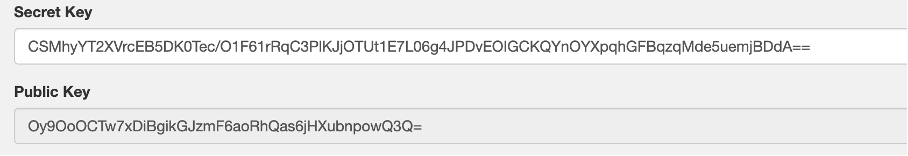
\includegraphics{F7_privatePublicKeys.png}
    \captionsetup{justification=centering, singlelinecheck=false}    
    \caption{De publieke en private sleutel voor encryptie aan de hand van TweetNaCL.js.}
    \label{fig:privatePublicKey}
\end{figure}}
 \newpage
In deze illustratie wordt een bericht dat afgebeeld staat hieronder \ref{fig:encryptionBericht} meegeven met de functie van TweetNaCl. Met als doel dit bericht te laten ondertekenen aan de hand van de geheime sleutel.

\begin{figure}[h]
    \centering
    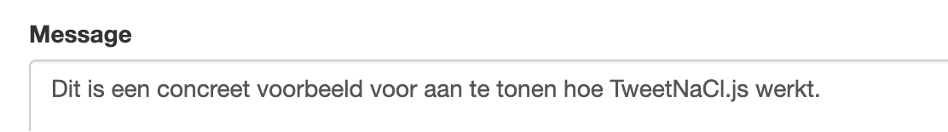
\includegraphics{F8_messageEncryption.png}
    \captionsetup{justification=centering, singlelinecheck=false}    
    \caption{Het bericht dat ondertekend moet worden encryptie aan de hand van TweetNaCL.js.}
    \label{fig:encryptionBericht}
\end{figure}}

Bij ondertekening van dit bericht ontstaat er een unieke handtekening  \ref{fig:signatureQrcode} als zijnde een tekenreeks. Aan de hand van deze code kan de ontvanger verifiëren dat het bericht gedurende de transactie niet gewijzigd is.

\begin{figure}[h]
    \centering
    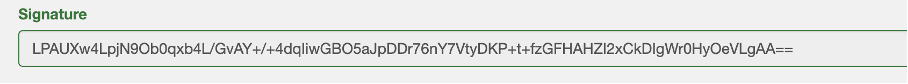
\includegraphics{F9_signature.png}
    \captionsetup{justification=centering, singlelinecheck=false}    
    \caption{De gegenereerde digitale handtekening aan de hand van TweetNaCL.js}
    \label{fig:signatureQrcode}
\end{figure}}

Om na te gaan of dit bericht zijn oorspronkelijke data bevat zal de functie ‘verify’ opgeroepen worden. In het geval dat dit bericht niet in oorspronkelijke status bevindt, zal de functie een foutboodschap retourneren \ref{fig:verifyFailed} . Als de methode geen foutboodschap weergeeft, kan men concluderen dat deze data origineel is \autocite{Bernstein2014}. Zoals word weergegeven in figuur \ref{fig:verified}.

\begin{figure}[h]
    \centering
    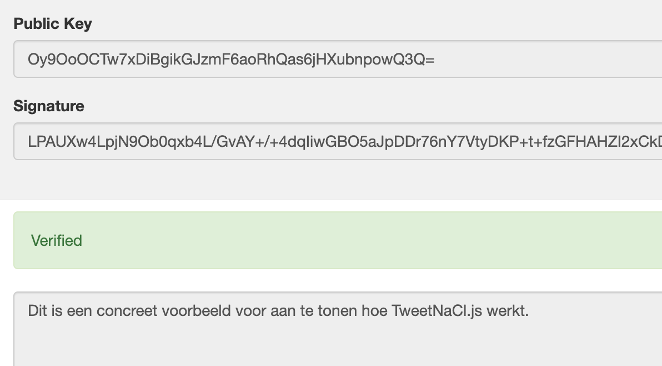
\includegraphics{F10_verified.png}
    \captionsetup{justification=centering, singlelinecheck=false}    
    \caption{Bewijs dat bericht zich in originele  staat bevindt.}
    \label{fig:verified}
\end{figure}}

\begin{figure}[h]
    \centering
    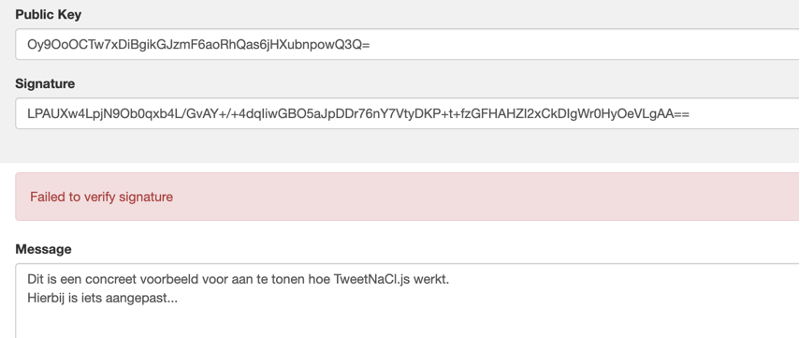
\includegraphics{F11_failedVerify.png}
    \captionsetup{justification=centering, singlelinecheck=false}    
    \caption{Bewijs dat bericht zich in geen originele  staat bevindt.}
    \label{fig:verifyFailed}
\end{figure}}
\\
\newpage
\newpage
\subsubsection{Uitgewerkt voorbeeld van digitale ondertekening op een aangemaakte QR-Code.}%
\label{sec:voorbeeldDigitaleSigningQRCode}

Bij de implementatie van deze smart locker technologie is het bericht dat standaard meegegeven wordt de QR-code data van type JSON object. Deze kan niet ondertekend worden zolang het niet geconverteerd wordt naar een tekstueel gegeven. De omvorming van een JSON object naar een string wordt verwerkt door de functie ‘deCodeBase64’. Deze functie zal de reeks decoderen terug naar het oorspronkelijke binair formaat \autocite{Josefsson2006}.

De functie ‘NaCL. Sign()’ aanvaardt twee parameters \ref{lst:encryptionCode}. In de eerste plaats nemen we de locker informatie op. Deze informatie beschikt over de locker nummer, creatiedatum QR-code en verval datum QR-code \ref{lst:essentieleQrdata}. Vervolgens heeft de functie een geheime sleutel nodig om de ondertekening te kunnen uitvoeren.

\begin{lstlisting}[caption={Data object met de naam smallItem bevat de essentiele data om een locker te openen.}, label={lst:essentieleQrdata}]
    export async function generateQrCodeWithRecord(qrData: {
        lockerNumber: any;
        start: number;
        end: number;
        color: string;
        image: string;
        location: string;
        name: string;
        periodName: string;
    }) {
        const smallItem = convertToSmallPayload(
        qrData.lockerNumber,
        qrData.start,
        qrData.end
        );
\end{lstlisting}

\begin{lstlisting}[caption={Digitale ondertekening van QR-code data.}, label={lst:encryptionCode}]
    const data = nacl.sign.detached(
    decodeUTF8(JSON.stringify(smallItem)),
    decodeBase64(
    'Hier komt de private key'
    )
    );
    \end{lstlisting}


Door de twee gecreëerde objecten, QR-data en de digitale handtekening samen te voegen ontstaat er een JSON object genaamd ‘createdCode’ \ref{lst:createCode}. De code wordt achteraf omgevormd naar een tekstueel formaat.

\begin{lstlisting}[caption={Samenstellen van object, locker informatie en verificatie code.}, label={lst:createCode}]
    const createdCode = Buffer.from(
    JSON.stringify({ d: smallItem, v: encodeBase64(data) })
    ).toString('base64');
\end{lstlisting}

Als illustratie maken we een QR-code aan op de applicatie die bestemd is voor locker nummer één. De geldigheidsduur van de code is tien minuten. Het request kan onderschept worden om zo de data te analyseren. We beelden het object af in figuur \ref{fig:dataobjectQR}

\begin{figure}[h]
    \centering
    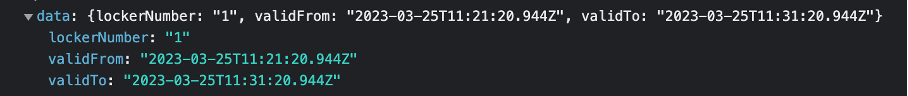
\includegraphics{F12_requestQrCode.png}
    \captionsetup{justification=ce/brntering, singlelinecheck=false}    
    \caption{Het data object bij de creatie van locker nummer 1 als logistieke medewerker. Deze heeft een tijdspanne van tien minuten.}
    \label{fig:dataobjectQR}
\end{figure}}

\newpage
Als we dieper in de materie duiken is de aangemaakte code zichtbaar als antwoord op het creatieverzoek. De tekstuele code voorgesteld als base64 string ziet er als volgt uit: \\
 “eyJkIjp7Im4iOiIxIiwiZiI6MTY3OTc0MzIyMSwidCI6MTY3OTc0Mzg4MX0sInYiOiJLYT
 cwTmg4WUo3RlY0NmNiKythNlN3b21vczFFVURiQlpxajl2ZDhpNlNUWGZHU003eVN
 2ZGw0ZEs5WGp3clpyVnNV RlpHR3E3RVJGSlJQR09HTkxEdz09In0=".
 
\vspace{7}

Deze code wordt achter een vaste ingestelde URL geplaatst zodanig dat de QR-code gemakkelijk gedeeld kan worden. Het delen of doorsturen van een QR-code is een eenvoudig proces voor de huurder. Als de QR-code gedeeld wordt een link gecreëerd dat verwijst naar de web applicatie van Lockit Rentals. De applicatie zal de base64 string die meegegeven wordt in de link ontcijferen en een afbeelding van de QR-code genereren.
